% QUESTAO
A figura abaixo é composta de dois quadrados de lado $x$, um quadrado de lado $y$ e um retângulo de lados $x$ e $y$.
\begin{center}
	\vspace{-3mm}
	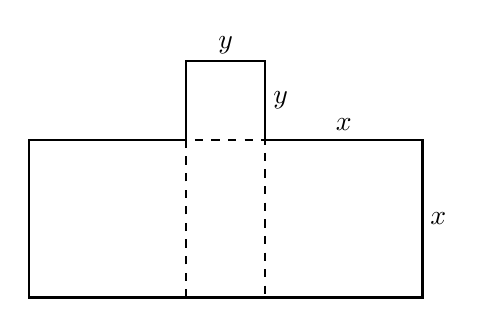
\begin{tikzpicture}
	\draw[thick] (0,0)--(5,0)--(5,2)--(3,2)--(3,3)--(2,3)--(2,2)--(0,2)--cycle;
	\draw[thick,dashed] (2,0) rectangle (3,2);
	\node at (4,2.2) {$x$};
	\node at (5.2,1) {$x$};
	\node at (2.5,3.2) {$y$};
	\node at (3.2,2.5) {$y$};
	\end{tikzpicture}
	\vspace{-3mm}
\end{center}
Quais as expressões algébricas que representam a área $(A)$ e o perímetro $(P)$ dessa figura?

% ALTERNATIVAS 7
$A=2x^2+xy+y^2$ e $P=6x+4y$
$A=3x^2-xy+y^2$ e $P=6x$
$A=x^2+2xy+y^3$ e $P=4y$
$A=2x^2-4xy+y^2$ e $P=10xy$
$A=4x^2+xy-y^2$ e $P=3x+2y$



